\chapter{背景と問題意識}
この章では、本研究における背景と問題意識について詳細に述べる。

\section{背景}
最初に、本研究の背景について述べる。

\subsection{IoT}
IoTとは、物理空間の様々なモノがネットワークに繋がり、そのデータに基づいて組織の意思や他のモノの動きが決定される世界の概念を表す言葉である。
特にこの一連の流れの際、人間が意図的にデータ入力をしたりデータ送信をしたりする必要がなく、これらをモノが自発的に人間にとってはシームレスに行うことをIoTという言葉で表す。
そしてこのIoTは我々の生活に大きな恩恵をもたらしている。
例えば既に販売されているサービスとして存在するものとして、道路事業者や交通事業者向けにその会社の自動車のGPS情報を取得し、交通情報を提示するものがある。\cite{hitachi_traffic}
これは、道路事業者が利用者に対する利便性の向上を、交通事業者が業務の効率化を測れるようにするものである。
また、自宅の外に温度センサ取り付けることでピンポイントで温度や湿度が取得でき、その情報をスマートフォンでスマートフォンから閲覧できる製品がある。\cite{thermometer}
これにより、屋外に出ることなく手元のデバイスですぐ外の気温を確認でき、例えば屋内で今日の服装を決定することができる。
このように、我々はIoTによって様々な利益を得ている。

この便利なIoTであるが、これの思想に基づいてサービスやアプリケーションを作り上げるには、コストのかかる工程が大きく分けて3つ存在する。
1つ目はSensing、情報を取得する必要がある。
交通情報の例では、各事業者の車にGPSを設置する部分がこれに当たる。
また、もしある交通事業者が直近に通っていない交通区間があったとすると、その区間の交通情報を取得することはできない。
温度計センサの例では、自分の家のすぐ外に温度計を設置する部分がこれに当たる。
2つ目はProcessing、情報を処理する必要がある。
交通情報の例では、GPSから取得した位置情報があまり変わっていないようであればそこが渋滞している可能性があると判断することがこれに当たる。
温度計の例では、特定の温度範囲を逸脱した場合、スマートフォンへ通知を送るようになっている部分がこれに当たる。
3つ目はActuation、情報を活かして行動する必要がある。
交通情報の例では、渋滞情報を地図上にマッピングしてわかりやすく提示することがこれに当たる。
温度計の例では、スマートフォンやPC上に温度を表示することがこれに当たる。
なお、ここで挙げた二つの例ではどちらもディスプレイに表示することがActuationに当たるが、他にも「工場内で温度上昇を検知した場合、工場内の生産機器の稼働率を下げる」ということを自動で行うこともこのActuationに当たる。
以上の流れは一般にSPA(Sensing、Processing、Actuationの略)と称され、これらを経てIoTの様々な製品やサービスは構築される。
また、これらの流れを図にしたものが下図\ref{SPA}である。
\begin{figure}[htbp]
 \centering
  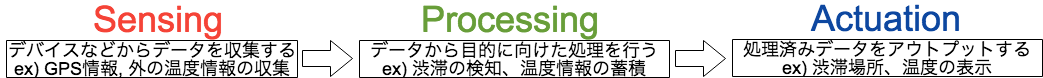
\includegraphics[width=140mm]{image/SPA.png}
 \caption{EverySenseにおけるIoTデータ市場イメージ}
 \label{SPA}
\end{figure}

\subsection{IoTデータ市場}
ところで、現状はSPAの処理を全て一つの主体が行う必要がある。
これら全てでIoTサービスが出来上がるので、当然と言えば当然だ。
しかし近年、これはIoTデータを売買できるプラットフォームである「IoTデータ市場」と呼ばれるものが出現している。
その中の一つがEverySense\cite{everysense}だ。
EverySenseはIoTデータを売買できるプラットフォームである。
このIoTデータ市場について、先の交通情報の例を使い、様々な観点から考えてみよう。
最初に、IoTデータの買い手の視点に立つ。
同じ道路を走る車にいくつものGPSセンサを取り付ける必要は、企業間の垣根を取り払えば存在しない。
同じ道路に同一事業者の車がいないので、その区間の交通情報を取得するためにセンサを取り付ける必要があるのだ。
もし他の会社の車のGPS情報を買い、取得することが出来れば、わざわざGPSセンサを取り付ける必要はない。
更に、先ほどは自社の車が通っていない交通区間についての情報を取得することはできなかったが、情報を買うことができれば通っていない道の交通情報も分かる。
次に、IoTデータの売り手の視点に立つ。
今まではGPSセンサを取り付けることは自社の為のみであった。
したがって、GPSセンサの代金や取り付けの工事費は全て自社のコストとなり、そのコストは顧客の払った売り上げから賄っていた。
しかしGPSセンサのデータが売れることが分かれば、このコストの一部はデータの買い手が負担することになり、価格面で顧客サービス向上につながる。
最後に、全体を俯瞰する観点に立つ。
同じ時刻に同じ場所を走行する別事業者の車両が1台ずつ、計2台が存在していたとする。
片方の会社はもう片方の会社から車両データを買えば良いので、IoTデータ市場の出現によって無駄なGPSセンサが1台減ることとなる。
更に、IoT化を進める上で不可欠なセンサが物理空間に増える可能性を孕んでいるのだ。
例えば、下図\ref{CarTraffic} \footnote{\url{https://ja.wikipedia.org/wiki/\%E4\%BA\%A4\%E9\%80\%9A\%E9\%87\%8F#/media/File:I-80_Eastshore_Fwy.jpg} (2018年1月23日確認)より引用、一部改変}のように異なる事業者によって、同じ道路を複数のカメラが同じように撮影する場合がある。
\begin{figure}[htbp]
 \centering
  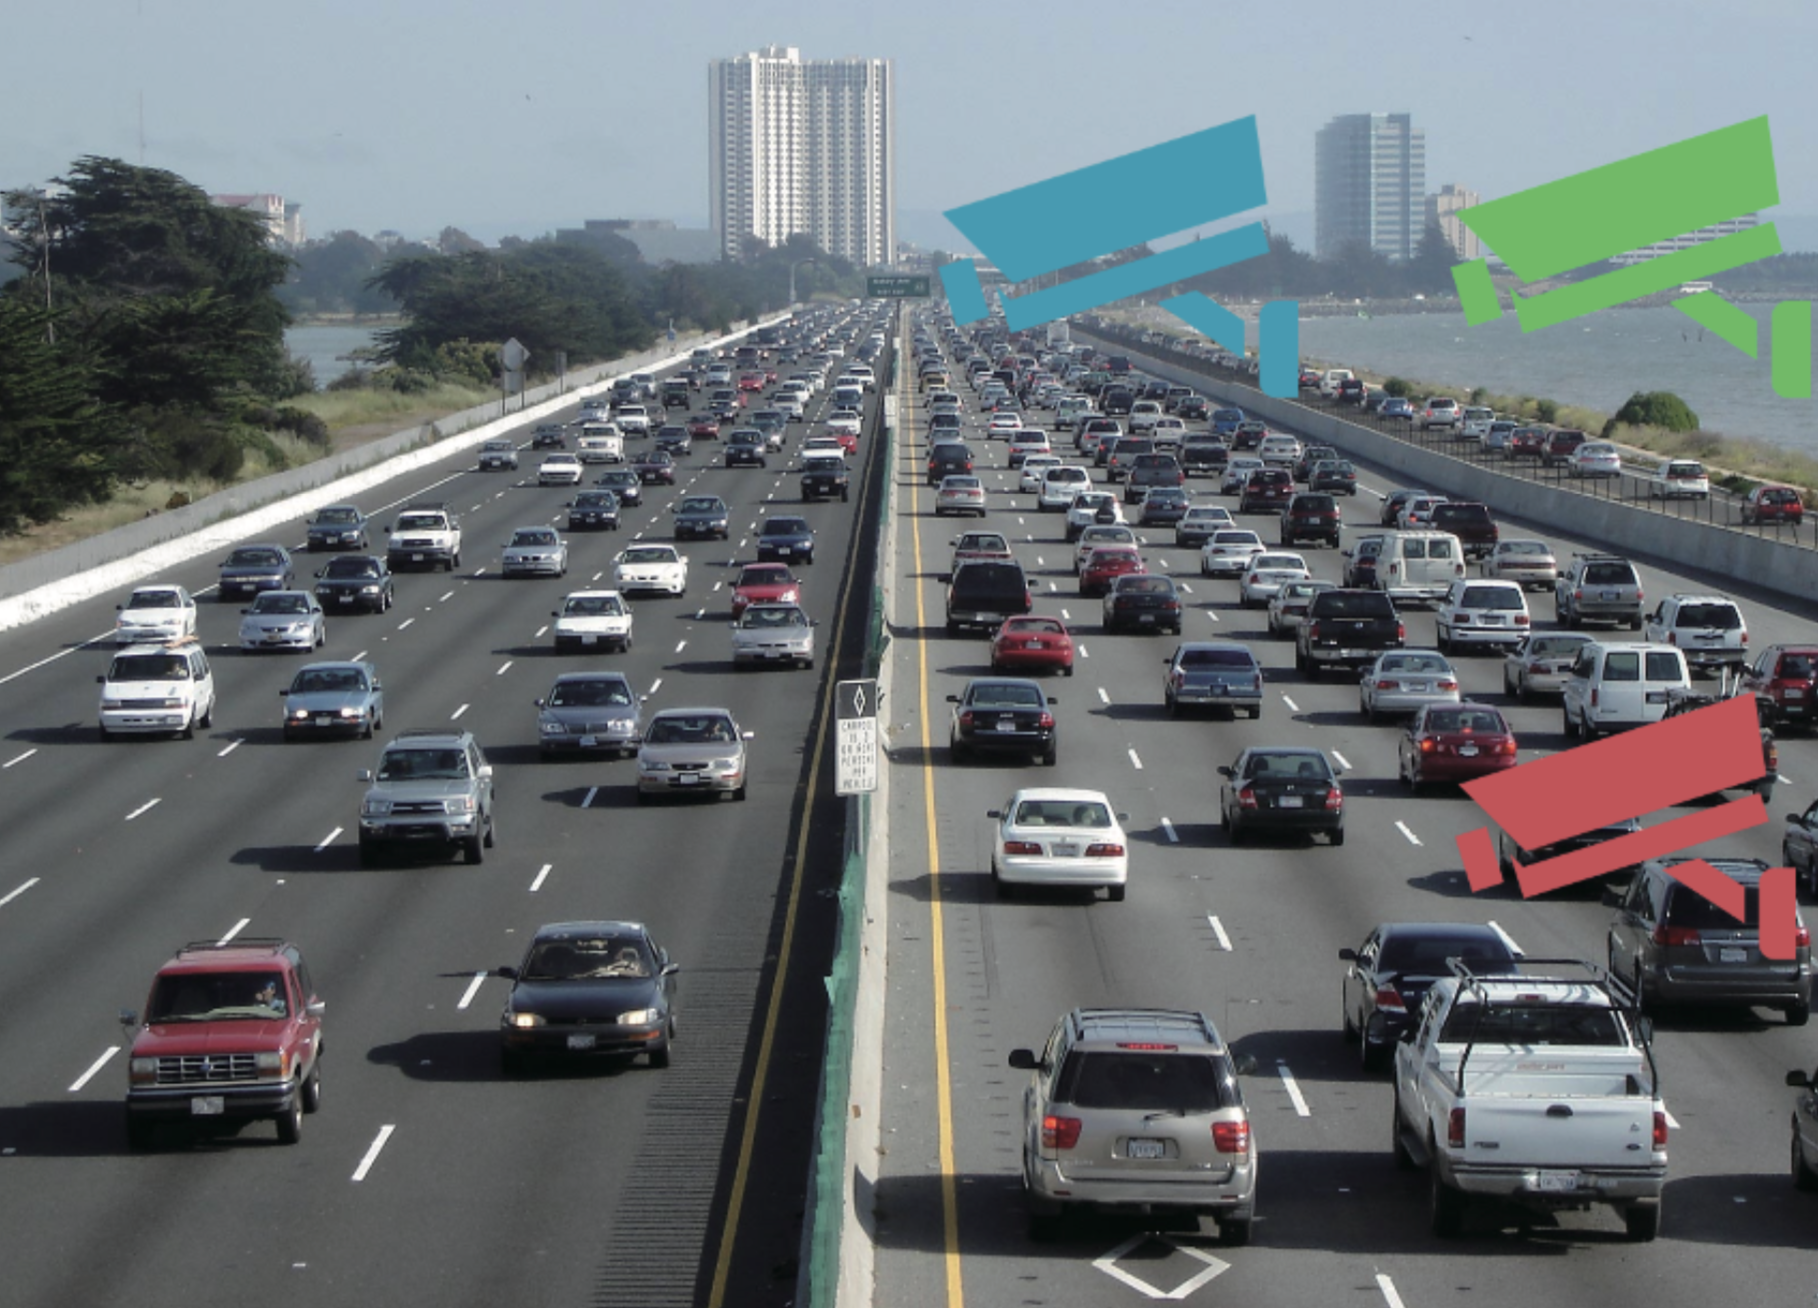
\includegraphics[width=100mm]{image/CarTraffic.png}
 \caption{複数のカメラが同じ道路の様子を撮影しているイメージ}
 \label{CarTraffic}
\end{figure}
データの売り手がデータ取得の費用が全て既存の顧客が払った売り上げから賄うわけではないと分かった場合、更に多くのセンサを車両に取り付ける可能性がある。
この時、世の中全体で使えるIoTセンサ量は増加し、世の中全体のIoT化が今までより容易に進むようになる。
このように、様々なステークホルダに利益をもたらし得るのがこのIoTデータ市場である。

\subsection{ブロックチェーン技術}
ブロックチェーン技術の詳細については後の3章にて述べるが、ここではこの技術の背景と概要について述べる。
詳細な理由については後述するが、IoTデータ市場は管理主体が存在しないほうが望ましい。
そして管理主体のいない市場を作る際は、その市場の金の流れについて全員が合意に達する必要がある。
この合意に達するためのアルゴリズムがブロックチェーン技術である。
合意アルゴリズムに関する研究は、現在最も有名なBitcoin\cite{Bitcoin}の開発以前も行われてきた。
完全に管理主体の存在しない研究として挙げられる'b-money'\cite{b-money}では、参加者の全員が受け取れる単一の歴史を示す元帳が必要であるとした。
これは現在のBitcoinをはじめとするブロックチェーンのアイデアの中心となるものである。
さらに、計算問題によって金を創造するという現在のブロックチェーンに使われているアイデアもこの論文にて導入されたが、提案が不十分であったため実装がなされなかった。
これらのアイデアをProof Of Workという具体的な手法で具現化し実装可能となり、作られたのがBitcoinであり、ここで使われている技術や後に更に考案された技術が総称されてブロックチェーン技術と呼ばれている。
現在ではチューリング完全で様々な暗号通貨の基軸暗号通貨プラットフォームとして使われているEthereum\cite{ethereum}やギャンブルのチップとして使われるAugur\cite{Augur}, 半中央集権的なRipple\cite{Ripple}などもこのブロックチェーン技術によって存在している。

\subsection{中央集権型サービスと分散型サービス}
一般に、中央集権的な管理者がいるサービスと管理者のいない分散型のサービスが存在し、各々で良い点と悪い点が存在する。 \\
管理者のいるサービスの良い点は、秩序が管理者を中心に整っていることである。
これにより、秩序の保守やサービスの変更といったサービス利用者にとって有意義な行動を簡単に取れるという利点がある。
例えばサービスの上で本来想定されていない使い方をしている、あるいは他人に迷惑をかける行為を行なっているといった管理者にとって悪いことをしているユーザを発見したとする。
この際、管理者がそのユーザのアカウントを凍結するなど、秩序を乱す原因となるものを素早く取り除くことができる。
また、新しい便利な機能を追加する時に、管理者がスピード感を持ってデプロイできる。
これは管理者が自分以外に合意を取るプロセスが不必要であるためである。 \\
一方、管理者がいないサービスの良い点は、そのサービスの透明性が担保されていることである。
管理者がいるサービスにおいて、管理者がユーザに対して不当に悪い扱いをしたとしても、その事実が表出しない。
例えばオンラインショッピングサービスの上で倫理的にも法律的にも正しく、商売を行っていたユーザがいるとする。
だがそのユーザの商売が、管理者も同じショッピングサービス場で行なっている商売と同じであり、管理者の利益を逼迫していたとする。
この時、管理者は悪い行いをしたユーザと同じようにそのユーザのアカウントを凍結することができる。
そしてこの事実を訴えたとしても、技術的にはアカウント凍結を覆すことはできない。
しかし、管理者のいないサービスがこのような事態を引き起こすことはない。
なぜなら全てのサービス利用者が対等な立場でサービスを利用するため、特定の利用者が大きな力を得ることがないためである。

\section{IoTデータ市場に関する問題}
IoTデータ市場は前述の背景を経て作られることとなったが、ここには問題点が存在する。
1.2節で述べたように、IoTデータ市場はIoTデータそのものの市場に対する寡占が発生しやすい市場である。
ここではその寡占状態になりやすい市場が中央集権的なサービスによって運営される際の問題点を、最初に政治的な問題点から述べる。
また、その後に技術的な問題点を述べるという方法で、2つに分けて説明する。

\subsection{政治的な問題}
最初に政治的な問題点について説明する。
政治的な問題、それは市場に単一の管理者が存在することだ。
そして単一の管理者は、その管理者の一存で市場を動かせるので、巨大な力を持つ。
そしてこの巨大な力は市場において2つの問題を孕んでいる。
1つ目は市場の管理者が市場の前提条件を簡単に覆せること。
2つ目は公正な市場の担保が難しくなること。 \\
1つ目、市場の管理者が市場の前提条件を簡単に覆せることについて考察する。
市場の管理者のビジネスモデルの代表的なものの一例としては、市場参加者がデータの売買をする際、プラットフォーム提供料として販売手数料を徴収する方法である。
この販売手数料が例えば10\%で設定されているとする。
すると、データの売り手は「10\%の販売手数料であれば例えばA円で販売し、このデータがBセット売れると考えられるのでA×B円が売り上げになる。そのためには~円のセンサを取り付けることによって最大の利益が得られる。」という計画で販売計画を立てる。
この販売計画の根底にあるものは「10\%の販売手数料」という前提である。
市場の管理者は他の誰の同意を得ることなしに、この10\%という値を30\%へ値上げすることが出来るのだ。
勿論、この値上げについては基本契約書での取り決めや、この市場に参加するまでのやりとりによっては参加者が法的に拒否することは可能である。
但し、法的に解決するには長い期間や訴訟のための費用がかかる上、今回のIoTデータ市場において司法がどのような判断を下すかは不明瞭である。
換言すると、管理者の存在がIoT市場において本格的に商売をしようとする事業者にとって信用する以外に方法のない存在であるのである。
つまり、この管理者が全ての善意のIoT市場の参加者にとって「正しく」機能する必要があるが、このことについて確実に担保する術は存在しない。
以上、市場の前提条件を覆せる可能性について言及した。 \\
2つ目、管理者の存在によって、公正な市場の担保が難しいという点について考察する。
IoTデータ市場は参加者にとって商機の存在するサービスであり、サービスを使うことに対して必死になる動機が十分にある。
このように参加者が必死になるサービスにおいて特定の管理者がいた場合、この管理者の持つ権限は巨大なものとなる。
例えばA社とB社がライバル関係であり、どちらも管理者のいる同じIoTデータ市場で商売をしていたとする。
この時、A社はB社に不利になるような、あるいはA社にとって有利になるような仕様の改変を求める可能性は十分にある。
更に管理者はその改変が出来てしまうので、仕様の改変を行う代わりに管理者がA社に対して見返りを求めることが可能になる。
この見返りを求められるような力を管理者は持ってしまっている。
そしてこのような状態は市場全体に対して良い影響を与えない。
自社のコストカットによる値段の抑制を行う、あるいは他者との差別化を図れるデータ収集を行って商機を図るといった正しい競争原理が働かなくなる。
権力者に近づくことが利益を上げる最善の手法となってしまうためだ。
更にIoTデータ市場は巨大な市場となりうるため、その権力者は更に大きな力を持ち、見返り目的に行動しやすくなる。
このような危険性は、市場という多くのビジネスの根幹に存在する場所において致命的なリスクである。
ここでは、IoTデータ市場における管理者の存在が公正な市場を担保することは難しいことを述べた。 \\
以上、管理者の存在によるIoTデータ市場の政治的な問題点を大きく分けて二つの観点から述べた。

\subsection{技術的な問題}
可用性とセキュリティの観点から、管理者の存在するIoT市場の問題点について述べる。
最初に、可用性の観点から述べる。
IoT市場は一瞬であろうと市場取引やデータ送信が止まる事は望ましくない。
だが、特定の一つの管理者のプラットフォーム上で動く以上、稼働率100\%を担保することは難しい。
例えば、クラウドサービスとして有名なAWS(Amazon Web Service)のEC2などの稼働率に関するSLA(Service Level Agreement)は最高で99.99\%である。
この99.99\%を割り込んだ場合、サービスクレジット率の10\%がこれからAWSの製品を使う上で使える金となる。
仮に稼働率をこのSLAの99.99\%とした時、1年間でAWSが稼働していない時間は52.56分である。
オンプレミス環境と比べて可用性に比較的信頼が置かれているクラウドでさえ、1年単位で考えると1時間弱程度のダウンタイムは仕方がないとAWSは考えている。
この1時間弱の間にどれほどの裁かれるべきデータ送信が滞るのか。
IoTデータは逐次飛んでくるものであるので、この時間の間に大量のデータ送信が滞ってしまうことは想像に難くない。
また今回はクラウドを想定したが、管理者がクラウドサービスを使い可用性を100\%に限りなく近づけるような努力がなされているかどうかは市場の参加者からはチェックすることができない。
このように逐次的に大量のデータが流れ、それが止まってしまうと大きな問題の起こるIoTデータ市場においては、単一の管理主体がその市場全体を管理することは望ましくない。
次に、セキュリティの観点から述べる。
当然、管理者であっても買っていないデータを勝手に閲覧することは許されない契約を、市場の参加者と管理者間で結ぶだろう。
ただ、それであっても管理者が売買データを見ることは技術的に可能である。
また、どの企業がどのようなデータを買っているかについても、管理者は全て見ることができる。
これは管理者が悪意を持っていない前提ならば問題のない話であるが、悪意を持っていた場合は参加している事業者のIoT戦略が全て管理者に筒抜けであることを意味する。
またセキュリティの脆弱性を突かれた場合、取引データが管理者のデータベースから抜かれた時には事業者間のプライバシーである取引履歴が、IoTデータが抜けれた時には販売価値のあるIoTデータがそれぞれ不特定多数の人間によって見られる可能性を含んでいる。
このように、単一の管理者が多くの流出を避けるべきデータを持つことはなるべくない方が良い。
以上2点について、単一管理者の存在するIoT市場の問題点について技術的観点から述べた。

\section{まとめ}
本章ではIoTが我々の生活の役に立っていることと、そのためにはデータが不可欠でその市場が誕生していることを述べた。
しかしそこには管理者がいるという政治的な、技術的な問題点が存在することを示した。
そしてこの状況を改善するために、ブロックチェーン技術というものがあることを示した。